\subsection*{9.3}
A firm maximizes revenue for a elastic demand curve by producing where MR = MC, known as the profit maximizing condition.\\
Producing where MR is less than MC is not profit maximizing.\\
Remember AC = $\frac{TC}{Q}$\\
TC = AC$\times$Q\\
AC*, the average cost where MR = MC, must be greater than the minimum.\\
$\pi$ = (P$^*$ - AC$^*$)Q
\begin{figure}[H]
    \centering
    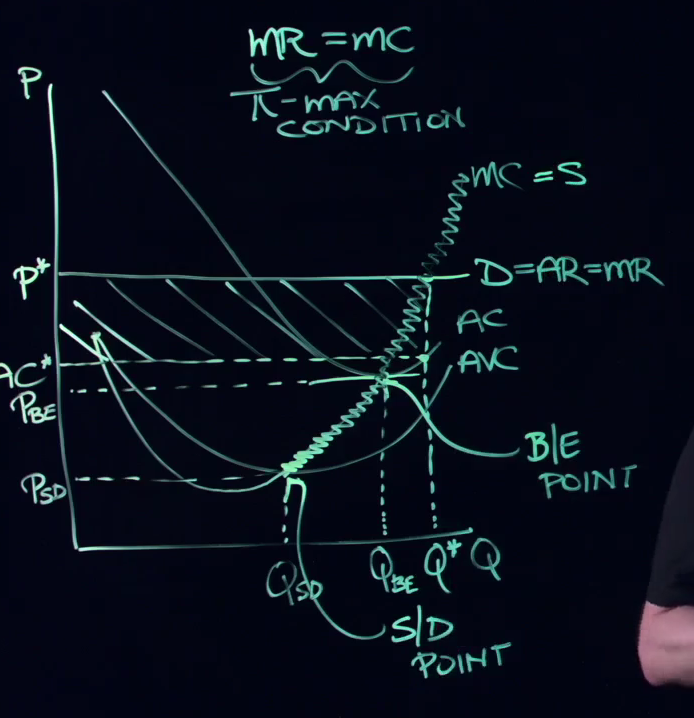
\includegraphics[width=0.5\textwidth]{./Chapter9/ProfitMaximization.png}
    \caption{Profit Maximization}
\end{figure}
The shaded area in the graph is the profits made.\\
If you have multiple intersection points, choose the rightmost.\\
If AC is greater than P, the firm is making a loss.\\
At a loss, the firm cannot pay all of their fixed costs.
\begin{figure}[H]
    \centering
    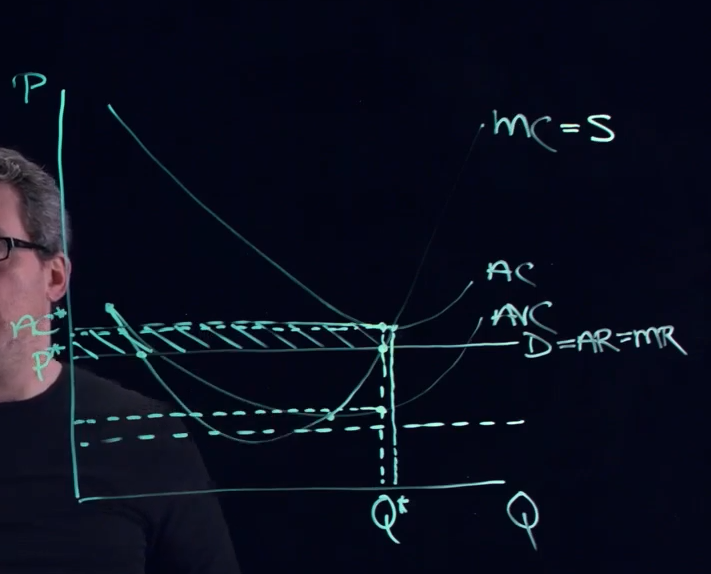
\includegraphics[width=0.5\textwidth]{./Chapter9/ProfitMaximizationLoss.png}
    \caption{Profit Maximization Loss}
\end{figure}
If the quantity at MR=MC intersects with the minimum of the AC curve, the firm breaks even.
This is known as the break even point, break even price and break even quantity.\\
Firms can lose so much money that they can't pay their variable cost.\\
If the quantity at MR=MC intersects with the minimum of the minimum of the AVC curve, this is the shut down point, shut down price and shut down quantity.\\
Marginal Cost curve is in fact the supply curve, as long as it is above the shut down point, otherwise the quantity supplied is 0. The reservation price is the shut down price.